\documentclass{projector}
% can use option mtpro 

\usepackage{psfrag}
% auto-pst-pdf permits psfrag to be used within the \begin{postscript} \end{postscript} environment. Only include it if you expect to use psfrag. Note that auto-pst-pdf does not work reliably with the \animategraphics command.
%\usepackage{auto-pst-pdf}
\usepackage{scalefnt}
% the package grffile is needed to read in graphics files that have more than 1 dot in the filename like DBD_actuator.T.1.pdf for instance
\usepackage{grffile}
\usepackage{bm}
\usepackage{booktabs}
\usepackage{animate}
\usepackage{graphbox}

\def\tlb{\\[0.2em]}
\def\ns{{n_{\rm s}}}
\newcommand{\alb}{\vspace{0.1cm}\\} % array line break
\renewcommand{\vec}[1]{\bm{#1}}

\ifdefined\postscript%
% if auto-pst-pdf package is included
  \let\oldpostscript\postscript
  \def\postscript{\oldpostscript\fontfamily{stix}\selectfont\scalefont{0.95}}
\else
% if auto-pst-pdf package is not included
  \def\postscript{\fontfamily{stix}\selectfont\scalefont{0.95}}
\fi%


\let\oldmath\math
\def\math{\oldmath\displaystyle}
\let\olddisplaymath\displaymath
\def\displaymath{\olddisplaymath}



\begin{document}

\squeeze


\begin{slide}
\centering
\vfill
\scalefont{1.8}
\textbf{Plasma Modeling for\\ Computational Aerodynamics}
\scalefont{0.6}
\vfill
Bernard Parent
\vfill
\emph{Pusan National University}
\vfill
\end{slide}





\begin{slide}
\Banner{Example of Plasma Aerodynamics:\\ Plasma Actuator on a Wing Segment}
\centering

\includegraphics[width=0.96\textwidth]{wing.jpg} 
\end{slide}




\begin{slide}
\Banner{Example of Plasma Aerodynamics:\\ Increase of Critical Angle of Attack}
\vfill
\begin{minipage}[c]{0.3\textwidth}
He et al., ``Plasma Flaps and Slats: An Application of Weakly Ionized Plasma Actuators'', \emph{Journal of Aircraft}, 2009.
\end{minipage}
\hfill
\begin{minipage}[c]{0.3\textwidth}
\includegraphics[align=t,width=1.0\textwidth]{flap.jpg}\\
Effect of plasma actuators on flow on top surface of flap.
\end{minipage}
\hfill
\begin{minipage}[c]{0.3\textwidth}
He et al., ``Plasma Flaps and Slats: An Application of Weakly Ionized Plasma Actuators'', \emph{Journal of Aircraft}, 2009.
\end{minipage}
\vfill
\end{slide}





\begin{slide}
\Banner{Lack of Detailed Numerical Results in Plasma Aerodynamics}
\vfill
\style{vskip=150}
    \begin{itemize}
      \item Many experiments demonstrate that plasma aerodynamics is viable    
      \item Preliminary numerical studies with simplified physical models also show that plasma aerodynamics is viable 
      \item Detailed numerical studies are still lacking    
      \item Because of this, plasma aerodynamics effects are incompletely understood  
      \item {\bf Why is simulating plasma aerodynamics in detail so difficult?}
    \end{itemize}
\vfill
\vfill
\end{slide}



\begin{slide}
\Banner{Aerodynamics Simulations vs\\ Plasmadynamics Simulations }
\style{vskip=110}
\vfill
\centering
\begin{tabular}{lll}
\toprule
 ~ & Aerodynamics  & Plasmadynamics   \\
Property& Simulations & Simulations \\ 
\midrule
Domain volume     &$\sim$ dm$^3$   & $\sim$ mm$^3$  \tlb
Length scale      & $\sim$ 10$^{-1}$ m  & $\sim$  $10^{-3}$~m   \tlb
Maximum drift speed      & $\sim$ 10$^3$ m/s  &  $\sim$ $10^6$ m/s \tlb
Time scale      & $\sim$ $10^{-4}$~s  & $\sim$ $10^{-9}$~s  \tlb
\bottomrule
\end{tabular}
\vfill
\flushleft
Aerodynamics simulations have {\bf time scales $\sim$5-order-of-magnitude higher} than  plasmadynamics simulations. 
\end{slide}







\begin{slide}
\Banner{Example of Plasmadynamics Simulation:\\ Discharge in Air Between Electrodes}
\vfill
   \centering
   \includegraphics[width=1.0\textwidth]{problem1.pdf}
\vfill
\end{slide}



\begin{slide}
\Banner{Air Discharge Case:\\ Electron Residual Convergence History}

\centering
   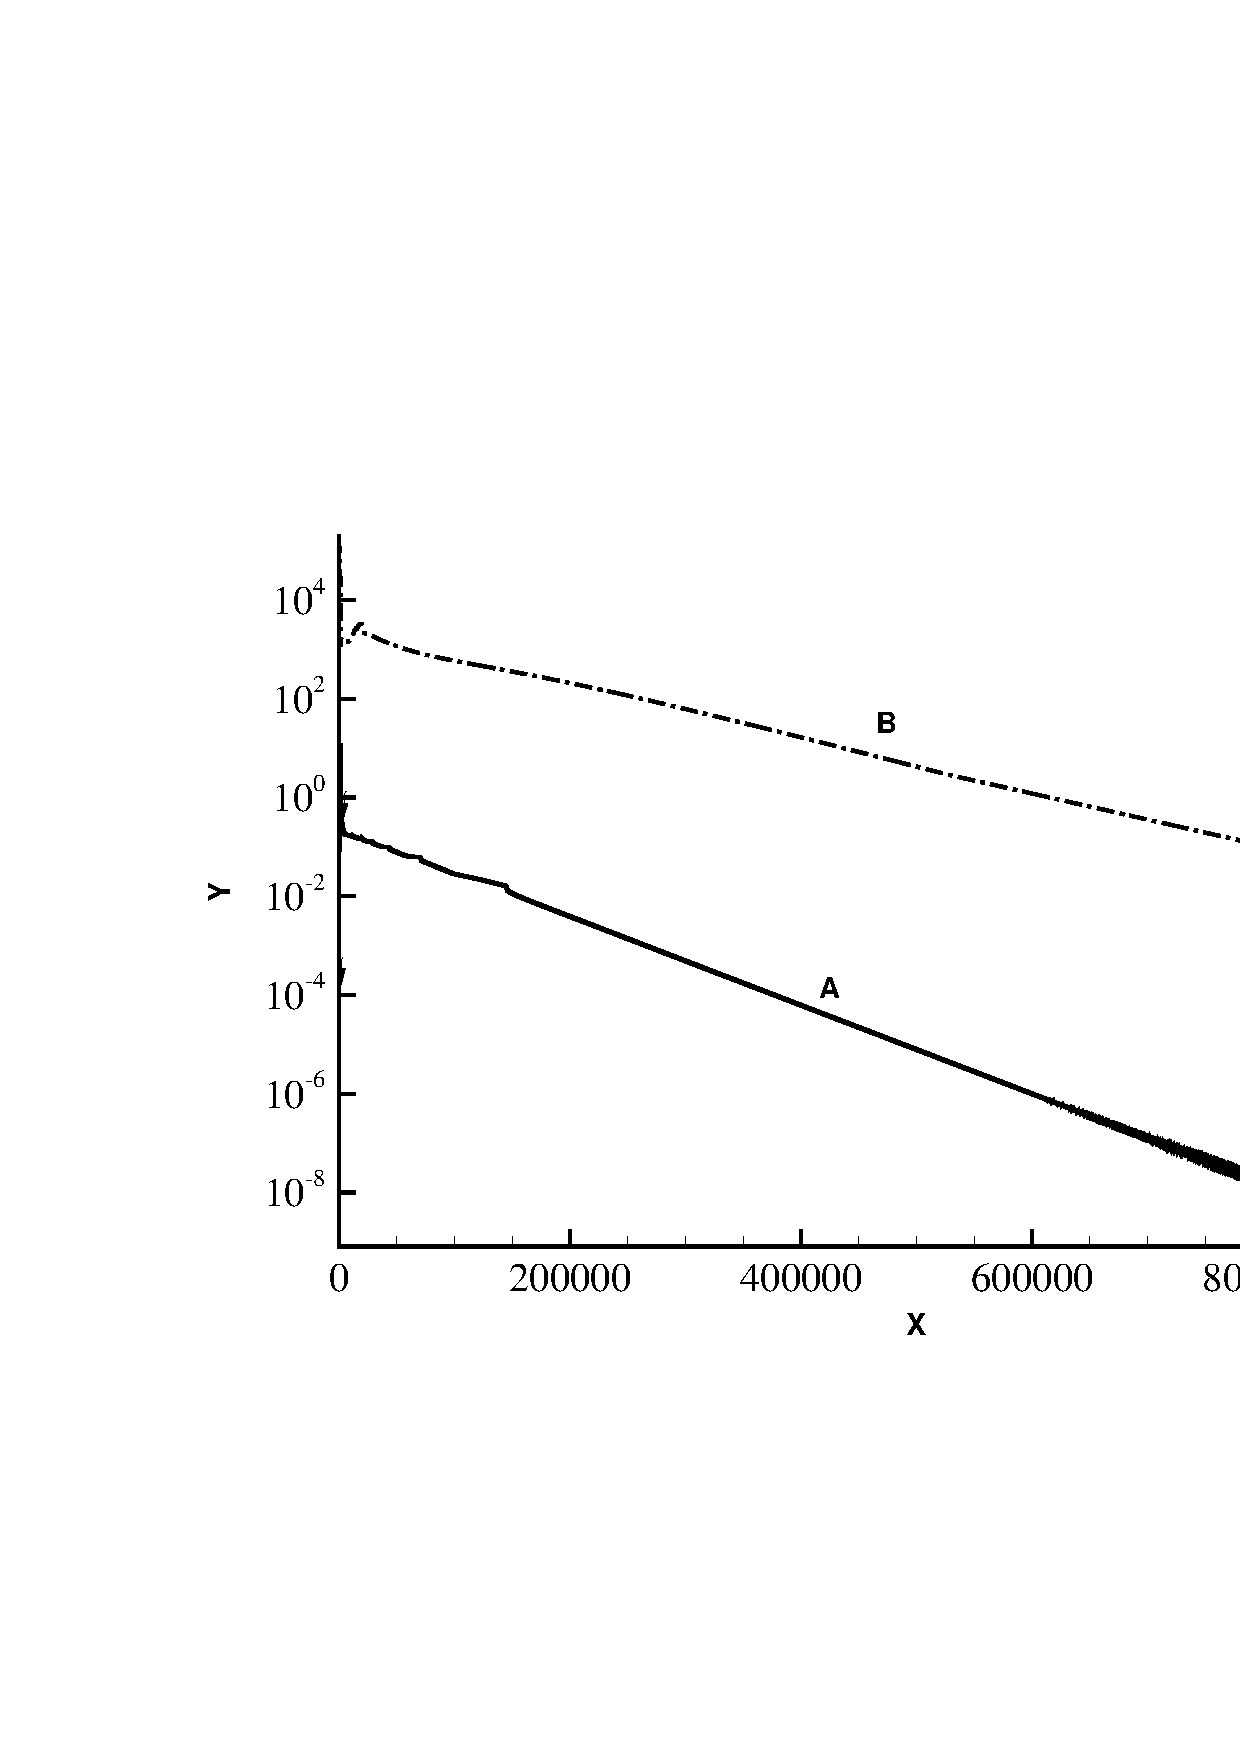
\includegraphics[width=0.9\textwidth]{case4-case6-ResNe.pdf}
\vfill
\flushleft
Equations exhibit \emph{high stiffness}: number of iterations is in the order of millions even when using a block-implicit scheme.
\end{slide}




\begin{slide}
\Banner{Current State of Plasma Modeling for Computational Aerodynamics}
\style{vskip=40}
\vfill
 {\bf Detailed plasma models:} 
         \begin{itemize}
            \item High stiffness
            \item Millions of iterations needed for convergence 
            \item \emph{Large numerical error} even with supercomputers
         \end{itemize} 
\vfill
 {\bf Simplified algebraic plasma models:}
         \begin{itemize}
            \item No stiffness
            \item \emph{Large physical error} for many problems of interest
         \end{itemize}
\vfill
 {\bf High-fidelity detailed simulations of plasma aerodynamics can't be accomplished with current supercomputers, numerical methods, and physical models.}
\vfill
\end{slide}



\begin{slide}
\Banner{How to Get Rid of the Stiffness?\\ Avoid Gauss-Based Potential}
\flushleft
\vfill
Replace Gauss-based potential equation:
\vfill
 \begin{math}
-\frac{\epsilon_0}{e} \, \frac{\partial^2\phi}{\partial x^2} =  N_{\rm i} - N_{\rm e}
\end{math}
\vfill
by a Ohm-based potential equation:
\vfill
\begin{math}
\frac{\partial }{\partial t}e(N_{\rm i}-N_{\rm e}) +  \frac{\partial}{\partial x} \left(  -\sigma \frac{\partial \phi}{\partial x}
             -   e D_{\rm i}  \frac{\partial N_{\rm i}}{\partial x}
             +   e D_{\rm e}  \frac{\partial N_{\rm e}}{\partial x}
\right) = 0
\end{math}
\vfill
which is obtained by summing the ion and electron transport equations multiplied by their respective charges.
\vfill
\end{slide}












\begin{slide}
\Banner{Non-Stiff Detailed Plasma Model\\ vs Conventional Detailed Model }
\vfill
\begin{itemize}
\item \emph{Disadvantage}
      \begin{itemize}
        \item Slightly more computing effort per iteration
      \end{itemize}
\vspace{0.8em}
\item \emph{Advantages}
      \begin{itemize}
        \item 30-100 times reduction in number of iterations
        \item up to 2 times increase in resolution along each dimension
        \item Possibility to use large ``aerodynamic-scale'' timesteps 
        \item Can be coupled with an aerodynamics solver 
      \end{itemize}
 \vfill\vfill
\end{itemize}
\end{slide}









\begin{slide}
\Banner{New Non-Stiff Detailed Plasma Model: Simulations Now Within Reach}
\vfill
\begin{itemize}
\item {\bf Detailed Simulations of Plasma-Assisted Combustion}
      \begin{itemize}
        \item Development of accurate plasma-fuel-air chemical models
        \item Simulations of combustor flows with plasma effects 
      \end{itemize}
\vspace{0.8em}
\item {\bf Detailed Simulations of Plasma Actuators}
      \begin{itemize}
        \item Large-Eddy Simulations (LES) including detailed plasma model 
        \item Investigation on the coupling between the plasma and the turbulence eddies  
      \end{itemize}
 \vfill\vfill
\end{itemize}
\end{slide}







\begin{slide}
\Banner{Heat Addition to Mach 2 Boundary Layer Using a DBD Actuator}
\centering
\vfill
\animategraphics[autoplay,controls,buttonsize=1em,poster=last,loop,width=0.86\textwidth]{8}{DBD_actuator_T.}{1}{34}
\end{slide}






\begin{slide}
\centering
\vfill\vfill\vfill
The slides shown today can be downloaded on
\vfill
{\bf http://bernardparent.ca}
\vfill
Thank you for coming to the seminar. 
\vfill\vfill\vfill
\end{slide}






\end{document}


%%%%%%%%%%%%%%%%%%%%%%%%%%%%%%%%%%%%%%%%%%%%%%%%%%%%%%%%%%%%%%%%
%% TEMPLATES





%%%% BLANK
\begin{slide}
\Banner{}
\vfill
\vfill
\end{slide}




%%%% FIGURE 
\begin{slide}
\Banner{}
\vfill
\centering
\includegraphics[align=b,height=0.6\textwidth]{???.pdf}
\vfill
\end{slide}




%%%% FIGURE AND CAPTION
\begin{slide}
\Banner{}
\vfill
\centering
\includegraphics[align=b,height=0.5\textwidth]{??.pdf}
\flushleft
\vfill
Caption
\vfill
\end{slide}





%%%% BIOGRAPHY
\begin{slide}
\Banner{}
\vfill
\includegraphics[align=t,width=0.3\textwidth]{??.pdf}
\hfill
\begin{minipage}[t]{0.65\textwidth}
      \begin{itemize}
	\item .. 
      \end{itemize}
\end{minipage}
\vfill
\end{slide}



%%%% Item list
\begin{slide}
\Banner{}
\vfill
\style{vskip=150}
\begin{itemize}
      \item 
    \end{itemize}
\vfill
\end{slide}




%%%% SIDE BY SIDE
\begin{slide}
\Banner{}
\vfill
\begin{minipage}[t]{0.45\textwidth}
%Text or figure on left side here
\end{minipage}
%or \includegraphics[align=t,width=0.45\textwidth]{flap.jpg}
\hfill
\begin{minipage}[t]{0.45\textwidth}
%Text or figure on right side here
\end{minipage}
\vfill
\end{slide}







%%%% PSFRAG 
%%%% Use only when the auto-pst-pdf package is included (see preamble)
%%%% Avoid psfrag unless absolutely necessary: better to use the bash script psfrag and create a pdf figure from tex and eps files
\begin{slide}
\Banner{}
\vfill
\begin{postscript}
   \psfrag{A}[l][l][1][0]{$a=b$}
   \includegraphics[width=0.7\textwidth]{file.pdf}
\end{postscript}
\vfill
\end{slide}



%%%% TABLE

\begin{slide}
\Banner{}
\centering
\vfill
\scalefont{0.94}
\begin{tabular}{lllll}
\toprule
Title1  & Title2 \\ 
\midrule
Item1     & Item2  \tlb
\bottomrule
\end{tabular}
\vfill\vfill
\end{slide}




%%%%% TWO FIGURES SIDE BY SIDE
\begin{slide}
\Banner{}

\vfill
   \includegraphics[align=c,width=0.48\textwidth]{figure1.pdf}\hfill %or \hspace{0.6em}
   \includegraphics[align=c,width=0.48\textwidth]{figure2.pdf}
\vfill
\end{slide}


%%%%% MOVIE
\begin{slide}
\Banner{Movie Title}
\centering
\vfill
\animategraphics[autoplay,controls,buttonsize=1em,poster=last,loop,width=0.86\textwidth]{8}{DBD_actuator_T.}{1}{34}
% the latter will include files named DBD_actuator_T.1.pdf, DBD_actuator_T.2.pdf, ..., DBD_actuator_T.34.pdf and play them at 8 frames per second 
% change the format of your png files to pdf with the command mogrify -format pdf DBD*png
\end{slide}



%%%% TITLE PAGE
\begin{slide}
\centering
\vfill
\scalefont{1.8}
\textbf{Seminar Title}
\scalefont{0.6}
\vfill
Your name
\vfill
\emph{Your Affiliation}
\vfill
\end{slide}





